\chapter{PENGUJIAN DAN ANALISIS}
Pada bab ini, akan dijelaskan mengenai hasil dari pengujian dan analisis dari penelitian yang telah diuraikan pada metodologi. Selain itu, akan dipaparkan mengenai skenario dari pengujian yang dilakukan untuk evaluasi performa dari sistem. Pengujian ini dilakukan untuk memastikan bahwa sistem yang telah dirancang mampu berfungsi dengan baik dan situasi yang mungkin dihadapi oleh pengguna.
\section{Skenario Pengujian}
Pengujian dilakukan untuk menguji performa dari model dalam melakukan deteksi terhadap gestur untuk sistem kendali dan sistem pengereman otomatis. Skenario pengujian dirancang untuk mengukur berbagai aspek dari sistem seperti akurasi deteksi terhadap kelas yang dipanggil, \emph{respond time}, kecepatan pemrosesan, dan respon sistem terhadap objek di depannya yang berpengaruh kepada pengereman otomatis. Skenario pengujian yang dilakukan adalah sebagai berikut;
\begin{enumerate}
    \item Hasil Pengujian model
    \item Pengujian berdasarkan FPS
    \item Pengujian berdasarkan hasil \emph{respond time}
    \item Pengujian terhadap akurasi dari kelas yang dipanggil
    \item Pengujian sistem pengereman otomatis pada jarak 150 cm
    \item Pengujian sistem pengereman otomatis pada jarak 130 cm
    \item Pengujian sistem pengereman otomatis pada jarak 100 cm
\end{enumerate}
\section{Pengujian Performa Model YOLOv11 Menggunakan Confusion Matrix}
Data yang digunakan sebagai set data berjumlah 5372 citra manusia dengan perbandingan 4359 set data train dan 1023 set data validasi. Setelah proses pemuatan set dilakukan di lanjutkan dengan proses pelatihan model.
Proses pelatihan dilakukan dengan beberapa parameter yang nantinya akan diuji, yang dimana parameter ini akan dibandingkan performanya melalui nilai confusion matrix maupun nilai akurasi deteksi seperti skor mAP, precision, box loss.
Gambar 4.1 merupakan input layer yang digunakan.
\begin{figure} [H] \centering
  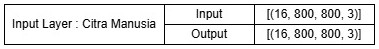
\includegraphics[scale=0.65]{gambar/Input layer.jpg}
  \caption{Input Layer Pelatihan}
  \label{fig:Pengujian Performa}
\end{figure}
Pelatihan pertama menggunakan 150 epoch. Input layer memiliki batch size sebesar 16 dengan tindakan praproses merubah ukuran gambar pada dataset menjadi 800x800 piksel. Adapun tujuan dari pelatihan ini untuk mengetahui seberapa baik peningkatan model pre- trained
yang digunakan dalam deteksi manusia berdasarkan jumlah Epoch yang ditentukan. Berikut nilai box loss yang didapatkan dari hasil training pada Gambar 4.2
\begin{figure} [H] \centering
  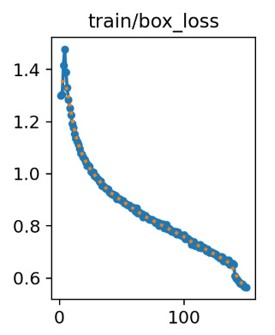
\includegraphics[scale=0.55]{gambar/train box loss.jpg}
  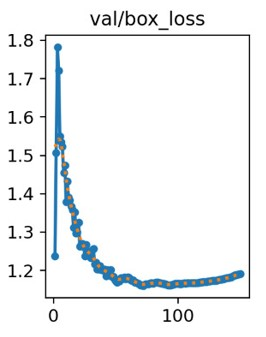
\includegraphics[scale=0.55]{gambar/val box loss.jpg}
  \caption{Grafik \emph{box loss}}
  \label{fig:Pengujian Performa}
\end{figure}
Didapatkan nilai dari \emph{box loss} pada hasil pelatihan YOLOv11 adalah sebesar 0.598
setelah 150 epoch. \emph{Box loss} mengukur seberapa baik model memprediksi bounding
box di sekitar objek. Tujuan dari loss ini adalah untuk mengoptimalkan model
agar bounding box yang diprediksi sesuai dengan posisi dan ukuran objek sebenarnya dalam gambar.
Adapun penurunan yang terlihat pada gambar pelatihan box loss menandakan bahwa hasil
pelatihan yang dilakukan telah berhasil membuat model menentukan koordinat \emph{bounding box}
pada objek manusia secara akurat.

Nilai dari \emph{box loss} pada proses validasi menggunakan YOLOv11 ini adalah 1.21,
\emph{box loss} validasi ini mengindikasi kemampuan mengenali objek pada data uji. Secara teori
, penurunan objek loss pada tahap validasi menandakan bahwa objek mampu melakukan deteksi
secara umum. Namun diakhir terlihat grafik sedikit naik. Hal ini menandakan ketika model
mulai menghafal pola data training dengan baik, tapi gagal menggeneralisasi pada data validasi.
Akibatnya, \emph{loss training} tetap atau terus menurun, loss validasi justru naik sedikit karena
model tidak mampu memprediksi data validasi dengan baik. Selanjutnya grafik dari mAP dapat dilihat
pada Gambar 4.3
\begin{figure} [H] \centering
  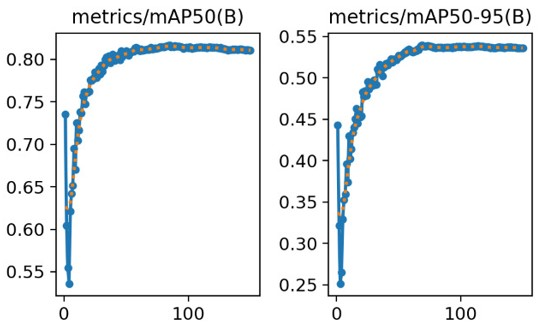
\includegraphics[scale=0.63]{gambar/map grafik yolov11.jpg}
  \caption{Grafik mAP epoch 150}
  \label{fig:Pengujian Performa}
\end{figure}
Skor mAP50 pada \emph{threshold} 0.5 yang diperoleh dari proses ini adalah sebesar 0.812, ini mengindikasikan
bahwa model memiliki kemampuan yang sangat baik dalam mendeteksi objek dengan kecepatan tinggi,
syarat minimal dari kriteria IoU adalah 0.5 terpenuhi. Hal ini menunjukan bahwa dalam percobaan kasus, \emph{bounding box}
yang diprediksi oleh model memiliki kesesuaian yang signifikan dengan \emph{bounding box ground truth}. 

Pada grafik mAP50-95 dengan prediksi yang lebih presisi. Nilai mAP50-95 adalah 0.25 diawal dan mulai terlihat kenaikan yang 
signifikan mencapai 0.543 di epoch ke 78. Hal ini menunjukan bahwa walaupun model sudah mampu mendeteksi objek dengan cukup
baik pada \emph{threshold} rendah, namun masih terdapat tantangan dalam mempertahankan akurasi deteksi
saat persyaratan presisi yang tumpang tindih semakin ketat.

Berikut merupakan grafik dari hasil yang didapatkan secara keseluruhan dari pealtihan model YOLOv11.
Pada Gambar 4.4 merupakan grafik hasil yang didapatkan pada model secara keseluruhan.
Didapatkan nilai- nilai pada masing masing grafik, pada train box loss didapatkan nilai 0.598,
pada train cls loss didapatkan nilai 0.412, pada train dfl loss didapatkan nilai 0.901 , pada
metrics precision didapatkan nilai 0.878, pada grafik recall 0.748, pada val box loss didapatkan nilai 1.211, pada val
cls loss didapatkan nilai 0.793, dan pada val dfl loss didapatkan nilai 1.342,  pada grafik mAP50
0.812, pada grafik mAP50-95 0.543

\begin{figure} [H] \centering
  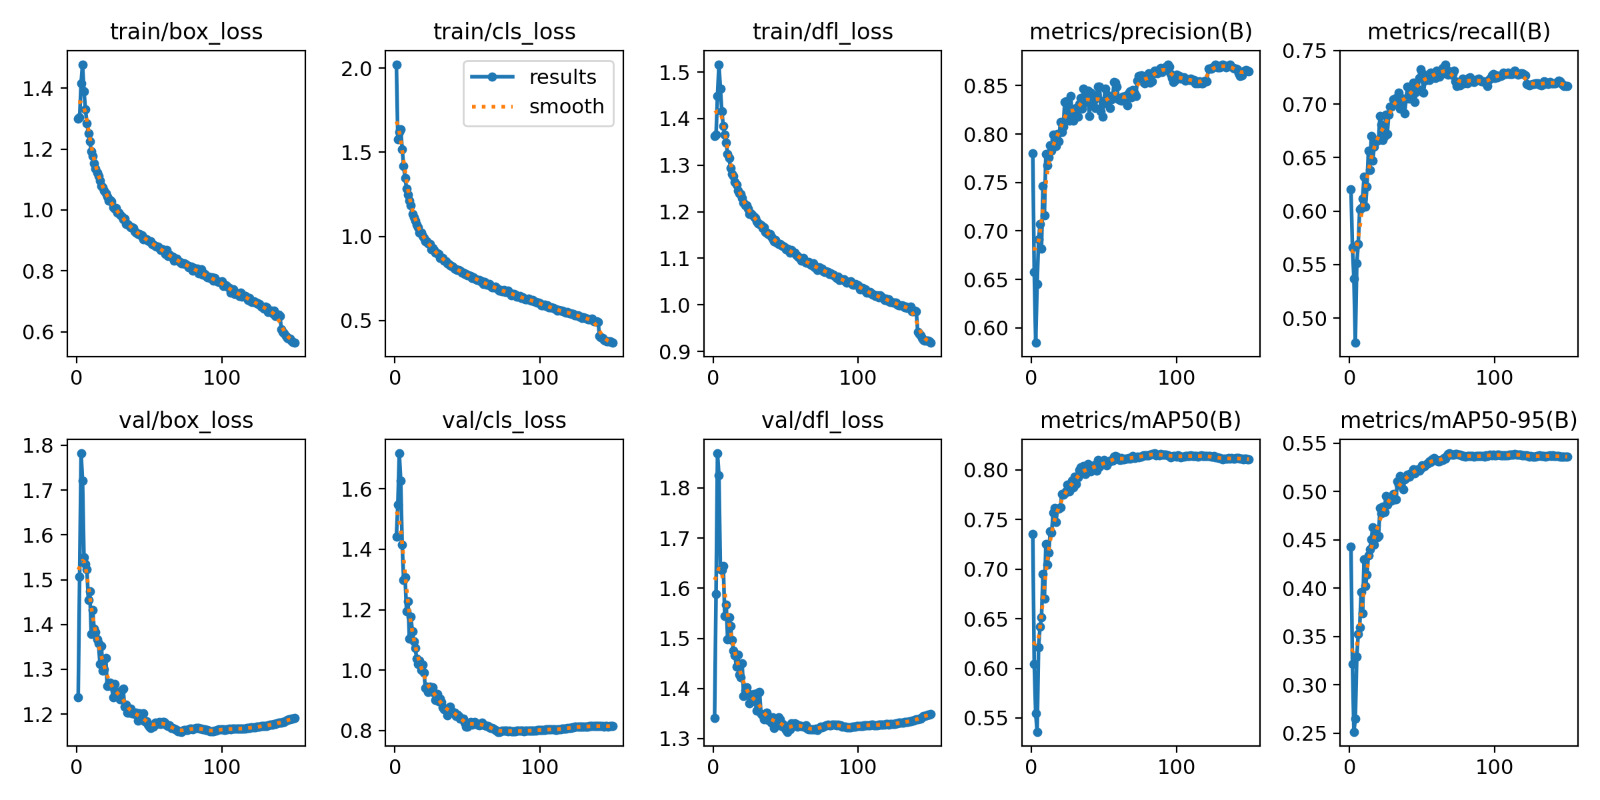
\includegraphics[scale=0.23]{gambar/Hasil.jpg}
  \caption{Grafik keseluruhan pelatihan epoch 150}
  \label{fig:Pengujian Performa}
\end{figure}

Berikut adalah visualisasi melalui \emph{confusion matrix} terkait dengan pelatihan model YOLOv11 dengan 150 epoch.
Pada Gambar 4.5 indikator yang digunakan pada \emph{confusion matrix} pada setiap kotaknya merepresentasikan nilai \emph{true positive, false positive, false negative, true negative}.
\begin{figure} [H] \centering
  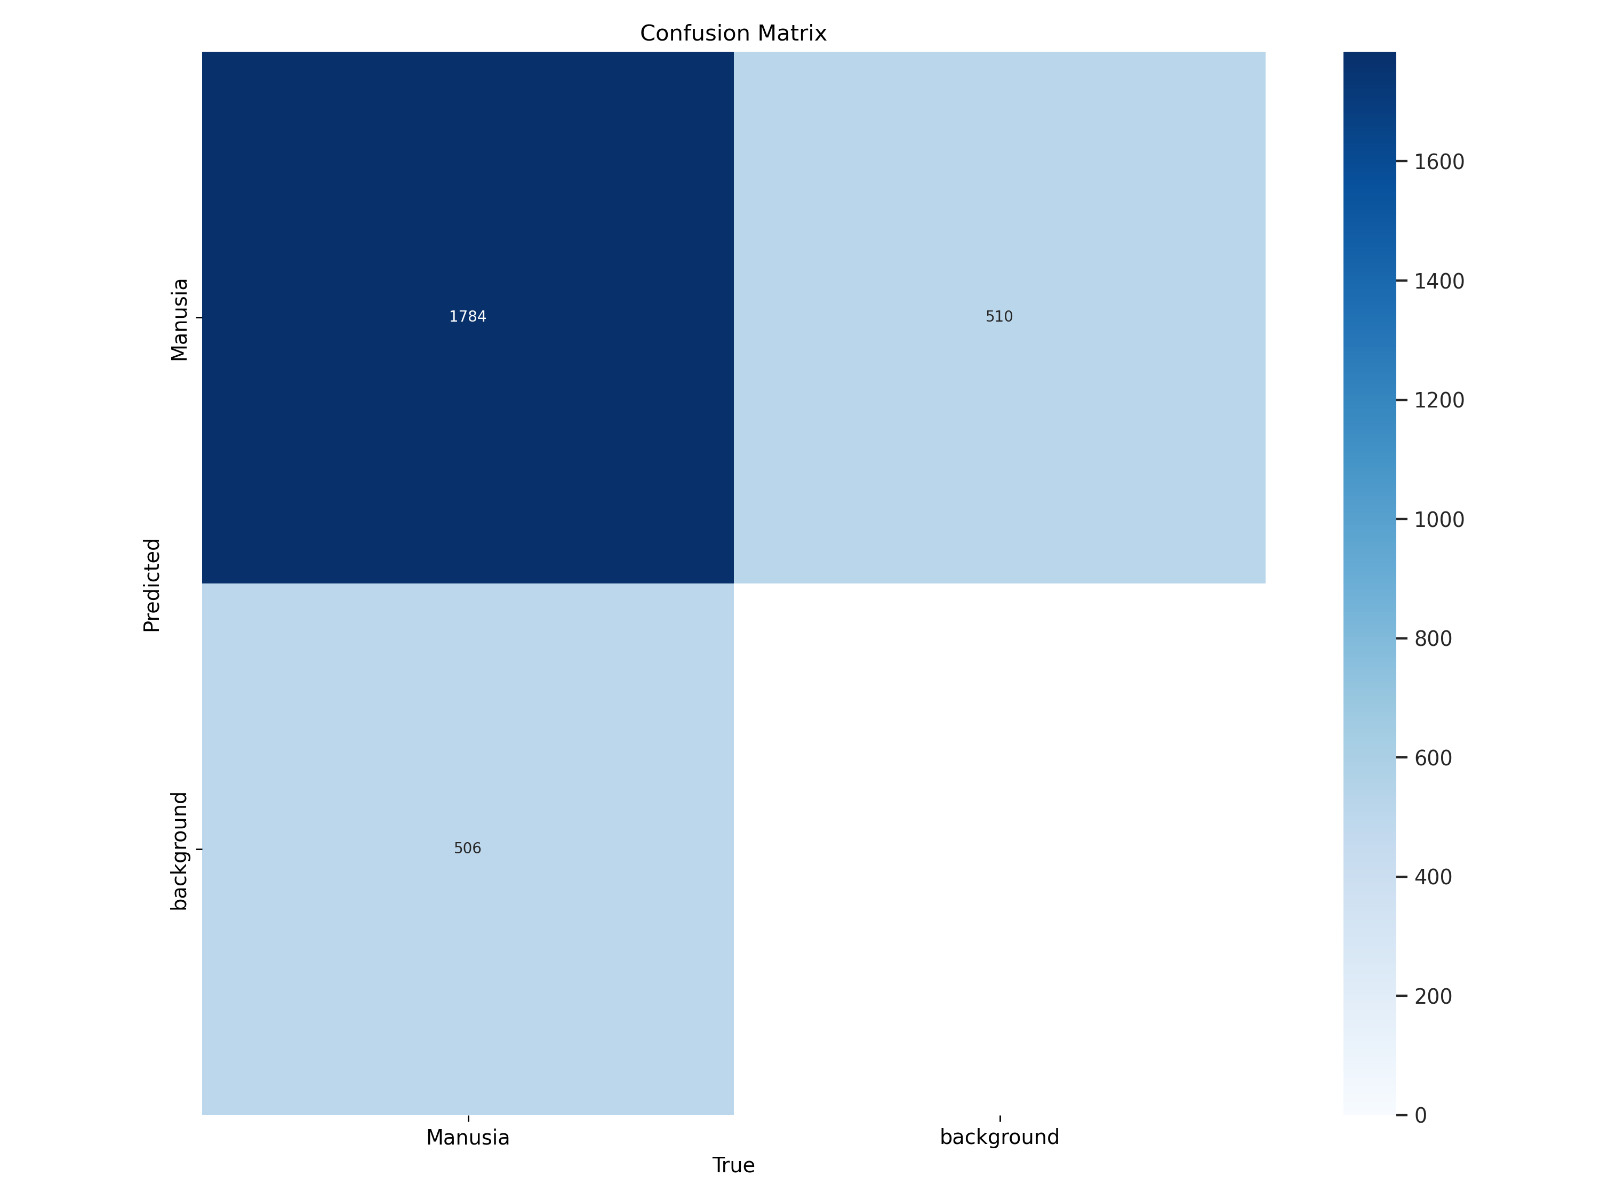
\includegraphics[scale=0.25]{gambar/Confusion matrix yolov11.jpg}
  \caption{\emph{Confusion matrix} pelatihan epoch 150}
  \label{fig:Pengujian Performa}
\end{figure}

Dari gambar 4.5 hasil pelatihan menunjukan dua kelas yakni manusia dan \emph{background}.
Dari hasil tersebut, model berhasil memprediksi hasil benar sebanyak 1784 sampel manusia. 
Namun, terdapat 510 sampel \emph{background} yang salah diklasifikasikan oleh model sebagai manusia. Disisi lain, model melewatkan 
506 sampel manusia yang diklasifikasikan sebagai \emph{background}. Selain itu, tidak ada prediksi yang benar-benar untuk kelas background,
yang mengindikasikan bahwa model cenderung memprioritaskan prediksi kelas manusia dan kurang mampu membedakan objek background dengan baik.
Hal ini menunjukkan adanya kecenderungan false positive dan false negative yang cukup signifikan

\section{Pengujian Performa Model LSTM Menggunakan Confusion Matrix}
Dataset untuk LSTM diambil dalam lima kelas dengan kelas yakni kelas kanan, stop, maju, mundur, dan kiri. Masing-masing kelas berjumlah 30 citra yang
telah di normalisasi tiap citranya, sebagai contoh pada gambar 4.6 merupakan gambar asli atau data mentah.
\begin{figure} [H] \centering
  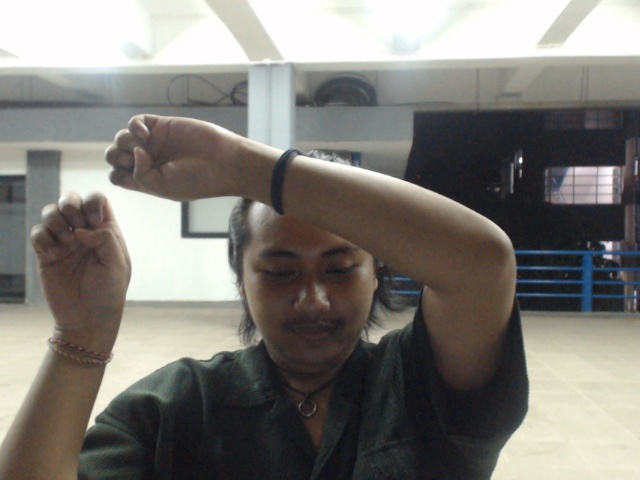
\includegraphics[scale=0.2]{gambar/0-clear.jpg}
  \caption{Dataset kelas kanan \emph{clear}}
  \label{fig:Data set kelas kanan raw}
\end{figure}

Kemudian pada gambar 4.7 menunjukan citra wajah dan tangan dengan titik-titik \emph{landmark} yang telah di deteksi menggunakan media pipe.
\begin{figure} [H] \centering
  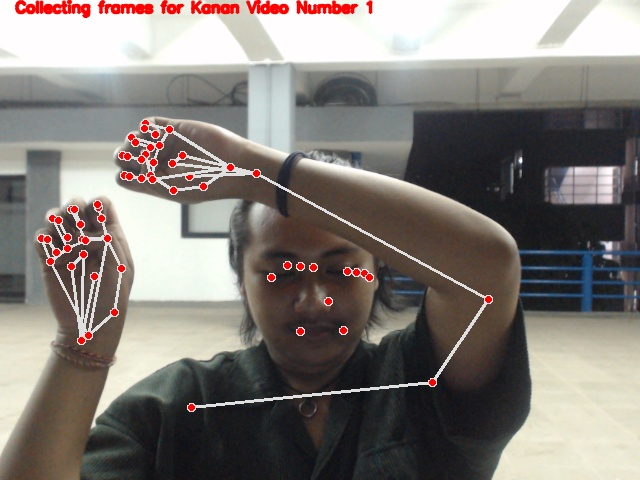
\includegraphics[scale=0.2]{gambar/1.jpg}
  \caption{Dataset kelas kanan \emph{landmark}}
  \label{fig:dataset kelas kanan clear}
\end{figure}
Dari gambar 4.7 diubah kedalam format .npy yang berisi data mentah dari titik-titik \emph{landmark}
yang terdeteksi pada bagian wajah dan dan tangan pada \emph{frame} video. File .npy ini berisi koordinat
2D dari landmark yang citra yang nantinya akan di normalisasi agar koordinat \emph{landmark} menjadi relatif 
terhadap gestur tangan sehingga data menjadi skala yang kosisten dan tidak bergantung pada ukuran asli dari citra. 
Normalisasi ini penting untuk memastikan model LSTM dapat belajar pola gestur tanpa terpengaruh perubahan ukuran citra atau posisi objek.
\begin{table}[htbp]
\centering
\caption{Tabel Sequencial}
\begin{tabular}{|l|l|l|}
\hline
\textbf{Layer (type)} & \textbf{Output Shape} & \textbf{Param \#} \\ \hline
time\_distributed (TimeDistributed) & (None, 30, 128) & 13,952 \\ \hline
lstm (LSTM) & (None, 30, 128) & 131,584 \\ \hline
dropout (Dropout) & (None, 30, 128) & 0 \\ \hline
lstm\_1 (LSTM) & (None, 30, 64) & 49,408 \\ \hline
dropout\_1 (Dropout) & (None, 30, 64) & 0 \\ \hline
lstm\_2 (LSTM) & (None, 32) & 12,416 \\ \hline
dropout\_2 (Dropout) & (None, 32) & 0 \\ \hline
dense\_1 (Dense) & (None, 16) & 528 \\ \hline
dropout\_3 (Dropout) & (None, 16) & 0 \\ \hline
dense\_2 (Dense) & (None, 16) & 272 \\ \hline
dropout\_4 (Dropout) & (None, 16) & 0 \\ \hline
dense\_3 (Dense) & (None, 5) & 85 \\ \hline
\end{tabular}
\end{table}

Tabel 4.1 menunjukkan ringkasan arsitektur model jaringan saraf yang terdiri dari beberapa layer berturut-turut. 
Dimulai dengan layer TimeDistributed yang menghasilkan output berukuran (None, 30, 128) dengan 13.952 parameter, 
yang berfungsi untuk menerapkan layer Dense pada setiap langkah waktu secara independen. Berikutnya terdapat tiga layer LSTM bertingkat, 
masing-masing dengan ukuran output (None, 30, 128), (None, 30, 64), dan (None, 32), serta jumlah parameter yang berkurang 
secara bertahap yaitu 131.584, 49.408, dan 12.416. Layer-layer ini menangani pemrosesan sekuensial data dengan mempertahankan urutan waktu 
dan mengekstrak fitur temporal yang kompleks. Setiap layer LSTM diikuti oleh layer Dropout yang tidak memiliki parameter, berfungsi sebagai 
regularisasi untuk mengurangi overfitting dengan mematikan sebagian neuron secara acak selama pelatihan. Setelah LSTM, model memiliki tiga 
layer Dense berturut-turut dengan ukuran output (None, 16), (None, 16), dan (None, 5) dengan jumlah parameter masing-masing 528, 272, dan 85. 
Layer Dense ini berfungsi untuk memetakan fitur yang telah diekstrak menjadi output klasifikasi akhir dengan 5 kelas, yang ditentukan oleh 
neuron pada layer terakhir.

Berdasarkan hasil akurasi \emph{training} yang telah dilakukan didapatkan bahwa model menghasilkan akurasi validasi bernilai 1 dan akurasi \emph{traininf}
bernilai 0.91. Data ini menunjukan peningkatan akurasi yang cukup baik pada data \emph{training} namun 
pada akurasi validasi mencapai 1.0 beberapa kali yang biasa jarang terjadi pada data validasi yang benar-benar baru dan representatif. Hal ini menandakan
data validasi terlalu kecil  atau kurang sehingga model mudah menghafal. Untuk nilai \emph{loss training} bernilai cukup tinggi di 2.56 dan \emph{loss} validasi di 
di nilai 0.05. Data ini menunjukan nilai \emph{loss training} secara umum menurun dari awal hingga akhir pelatihan, yang berarti model semakin baik dalam 
meminimalkan kesalahan terhadap data \emph{training} seiring dengan berjalannya \emph{epoch}. Untuk \emph{loss} validasi juga menunjukan tren penurunan yang konsisten. 
Hal ini mengindikasikan bahwa model dapat belajar dari data \emph{training} dengan cukup baik. Berikut merupakan grafik dari model akusari dan model \emph{loss} dari pelatihan model LSTM.
\begin{figure} [H] \centering
  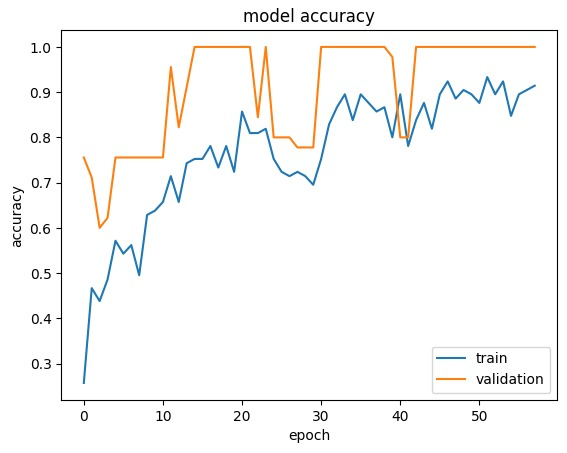
\includegraphics[scale=0.5]{gambar/akurasi model.jpg}
  \caption{Hasil \emph{accuracy} model LSTM}
  \label{fig:Pengujian Performa akurasi lstm}
\end{figure}
\begin{figure} [H] \centering
  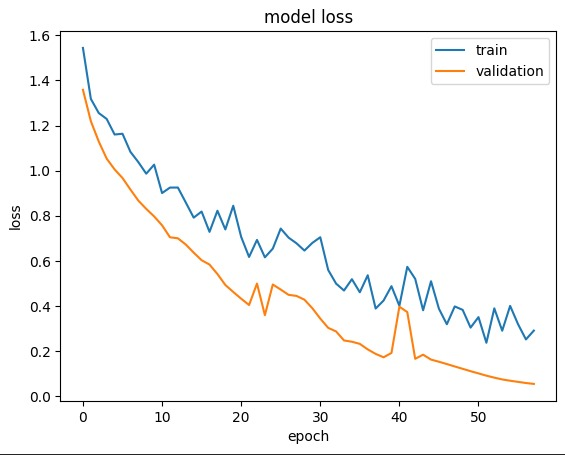
\includegraphics[scale=0.5]{gambar/akurasi loss.jpg}
  \caption{Hasil model \emph{loss} LSTM}
  \label{fig:Pengujian Performa model loss lstm}
\end{figure}

Kemudian berdasarkan model yang telah dilatih, dilakukan pengujian dengan dataset \emph{testing} yang menghasilkan \emph{confusion matrix}.
Gambar 4.10 menunjukkan confusion matrix dari sebuah model klasifikasi dengan lima kelas yaitu Stop, Maju, Mundur, Kanan, dan Kiri. Dari matriks ini dapat dilihat bahwa model mampu
mengklasifikasikan setiap kelas dengan sangat baik tanpa terjadi kesalahan prediksi antar kelas. Misalnya, untuk kelas Stop, seluruh 11 sampel diklasifikasikan dengan benar sebagai Stop, 
dan hal yang sama berlaku untuk kelas Maju dengan 11 sampel yang benar, kelas Mundur dengan 9 sampel, serta kelas Kanan dan Kiri yang masing-masing diklasifikasikan benar sebanyak 7 sampel. 
Tidak terdapat nilai selain diagonal utama yang berarti tidak ada sampel yang salah diklasifikasikan ke kelas lain. Hal ini menunjukkan performa model yang sangat akurat dalam mengenali kelima kelas tersebut. 
\begin{figure} [H] \centering
  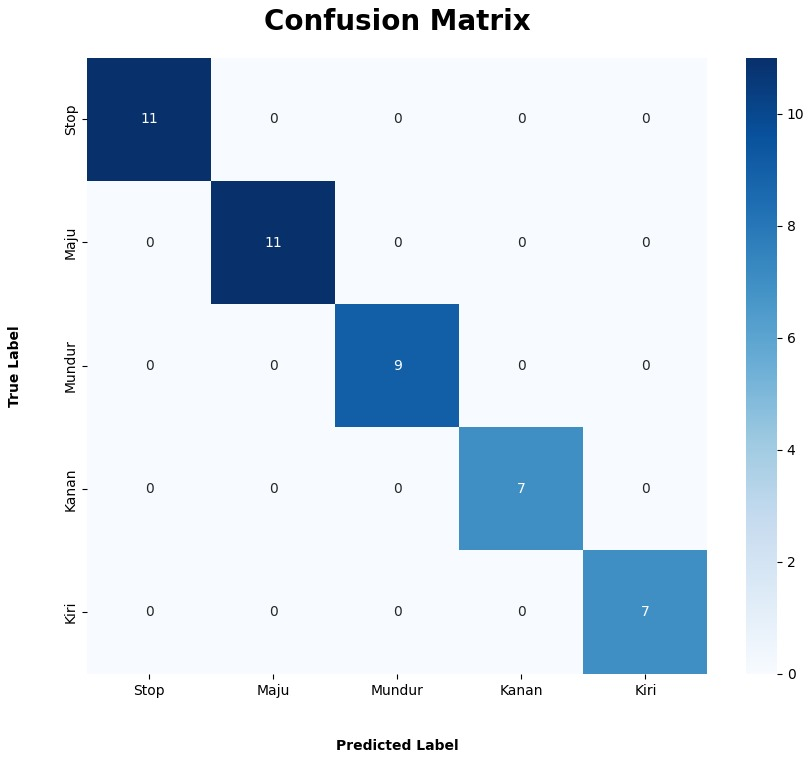
\includegraphics[scale=0.5]{gambar/confusion matrix lstm.jpg}
  \caption{Hasil \emph{confusion matrix} LSTM}
  \label{fig:Grafik confusion matrix lstm}
\end{figure}

\begin{table}[h!]
\centering
\caption{Classification Report}
\begin{tabular}{lcccc}
\hline
\textbf{Class} & \textbf{Precision} & \textbf{Recall} & \textbf{F1-score} & \textbf{Support} \\
\hline
Stop   & 1.00 & 1.00 & 1.00 & 11 \\
Maju   & 1.00 & 1.00 & 1.00 & 11 \\
Mundur & 1.00 & 1.00 & 1.00 & 9  \\
Kanan  & 1.00 & 1.00 & 1.00 & 7  \\
Kiri   & 1.00 & 1.00 & 1.00 & 7  \\
\hline
\textbf{Accuracy}     & \multicolumn{4}{c}{1.00} \\
\textbf{Macro avg}    & 1.00 & 1.00 & 1.00 & 45 \\
\textbf{Weighted avg} & 1.00 & 1.00 & 1.00 & 45 \\
\hline
\end{tabular}
\end{table}

Tabel 4.2 menunjukkan hasil evaluasi model klasifikasi untuk lima kelas, yaitu Stop, Maju, Mundur, Kanan, dan Kiri. Dari tabel tersebut terlihat bahwa model mencapai nilai precision, recall, dan f1-score sebesar 1.00 pada semua kelas, 
yang berarti model mampu mengklasifikasikan setiap kelas dengan sempurna tanpa kesalahan. Support menunjukkan jumlah data uji pada masing-masing kelas, dengan total 45 sampel yang tersebar di kelima kelas tersebut. Nilai accuracy sebesar 1.00 
mengindikasikan bahwa model memiliki akurasi 100\% secara keseluruhan pada data uji ini. Selain itu, nilai macro average dan weighted average yang juga 1.00 memperkuat bahwa performa model sangat baik dan konsisten di seluruh kelas.